\chapter{Suscriptor de Podcast}

\section{Tecnologías de la información y comunicación}

Se denomina Tecnologías de la Información y Comunicación (TIC) a la radio,
televisión e Internet brindan soporte de recuperación de información
y la presentan para la sociedad.

\subsection{Tecnologías de la información y comunicación en la educación}

Las TIC ayudan a diversificar la enseñanza y el aprendizaje de las lenguas
originarias y extranjeras. Debido a esta ventaja que proporciona varios
países de América latina y el Caribe optan por implementar políticas
gubernamentales de promoción de las TIC y de equipamiento a instituciones
públicas.

\section{Web 2.0}

La web 2.0 se denominada un sistema de principios y prácticas de comunicación y
servicios: facebook, flicker, youtube, blogger, twitter sobre la red de Internet.
Otro rasgo de la web 2.0 tiene la característica de compartir información entre
los usuarios, realizar comentarios respecto a un recurso y la evaluación la
realiza los propios usuarios. 

\section{La creación de contenido digital educativo}

Hay que mencionar que, la elaboración de contenido digital educativo requiere el
trabajo de profesionales de diferentes áreas, además la comunicación de los
profesionales necesita de uso de estándares para establecer etapas de trabajo.

De la misma manera la elaboración de material didáctico en soporte web
realiza la participación de al menos cuatro disciplinas. La primera es la
tecnología, que acostumbra a tomar la forma concreta de la informática. La
segunda es el diseño gráfico. La tercera es la pedagogía, y más la
especialización en tecnología educativa. La cuarta es, finalmente la lingüística.
\cite{duart2000aprender}

\subsection{Podcast}

El podcast es un archivo digital que tiene las siguientes características: un
reproductor (audio/vídeo), disponible en la web con la opción para descarga.

El podcast es un recurso o herramienta novedosa y muy útil por sus
características en el aprendizaje de una lengua. En el ámbito educativo el
podcast \textquotedouble{es una herramienta muy flexible para la educación
porque permite elaborar guiones adaptados a nuestra realidad educativa}
\cite{chacon2011podcast}. Es un recurso que permite hacer uso de la
creatividad en la producción de guiones con diferentes temáticas.
\cite{AFSTVV2014}

Se debe agregar que el término podcasting es la acción de crear un podcast y
realizar su difusión en la red de Internet.

\section{\textquestiondown Qué es un feed de noticia?}

La tecnología \footnote{tecnología: Es la aplicación de un conjunto de
conocimientos y habilidades con un claro objetivo: conseguir una solución que
permita al ser humano desde resolver un problema determinado hasta el lograr
satisfacer una necesidad en un ámbito concreto. \cite{technology}} feed
\footnote{feed: Un archivo coherente, legible por la máquina que
permite a los sitios web para compartir su contenido con otras aplicaciones en
una forma estándar.\cite{hammersley2005developing}} de noticia
actualiza al usuario a los últimos contenidos de un sitio web vía correo
electrónico. Esta tiene la siguiente estructura de título, descripción y
categoría.

Además el uso de RSS \footnote{RSS: Es un método de noticias descubriendo
un otro contenido Web que está disponible para la alimentación.
\cite{zeki2004rss}} y atom es proporcionar un feed de sindicación de
contenido un archivo coherente, legible por la máquina que permite a los
sitios web compartir su contenido con otras aplicaciones de manera estándar. \cite{hammersley2005developing}

Se debe agregar que RSS como formato basado en XML \footnote{XML: Es un
metalenguaje para definir idiomas para el intercambio de información en la
Web, los formatos de fuentes son también a menudo se llama
\textquotedouble{dialectos XML} o \textquotedouble{XML vocabularios}.
\cite{wittenbrink2005rss}} utiliza como estructura un suscriptor de noticia.

Es así que RSS y atom son documentos XML; tienen la función de actualizar y
compartir información. Este documento también es denominado newfeeds o feed.
\cite{wittenbrink2005rss}

\section{\textquestiondown Cómo indicar la existencia de un feed?}

Se identifica un ícono de color naranja, tiene en su interior un circulo y
dos lineas curvas de color blanco; a continuación, se da a conocer que la
aplicación web cuenta con un suscriptor.

\begin{figure}[h!]
\centering
	\fbox{
		
\includegraphics[scale=0.8]{rss}
	}	\caption{Ícono representación gráfica de un feed}
	\source{fuente: \cite{iconRss}}
	\label{fig:Ícono representación gráfica de un feed}
\end{figure}

\subsection{Información básica de un RSS 2.0}

Un suscriptor tiene un channel \footnote{channel: En las telecomunicaciones
en general un canal es un camino separado a través del cual las señales pueden
fluir. \cite{channel}} el cual debe incluir (items) título, enlace y
descripción. Estos elementos son obligatorios dentro un channel porque son
necesarios para caracterizar la recogida de información. El título del mensaje
es individual corresponde con el subtítulo en un archivo de tipo HTML 
\footnote{HTML:Es el conjunto de símbolos de marcado o códigos insertados en
un archivo destinado a la visualización de una página Web Mundial. \cite{html}},
que puede ser marcado como un elemento h2 o h3. El enlace feed utiliza el URI
\footnote{URI: Uniform Resource Identifier es la forma de identificar
cualquiera de esos puntos de contenido, ya sea una página de texto, un vídeo
o un clip de sonido, una imagen fija o animada, o un programa. \cite{uri}}
; que se especifica en el link (enlace) para crear un hipervínculo para el
documento. La especificación define vagamente como una \textquotedouble{frase
u oración que describe el channel}. \cite{wittenbrink2005rss}

En la figura \ref{fig:Estructura de un documento RSS simple como un diagrama de árbol},
la estructura de un documento RSS se representa de forma gráfica.

\begin{figure}[h!]
	\centering
	\fbox{
		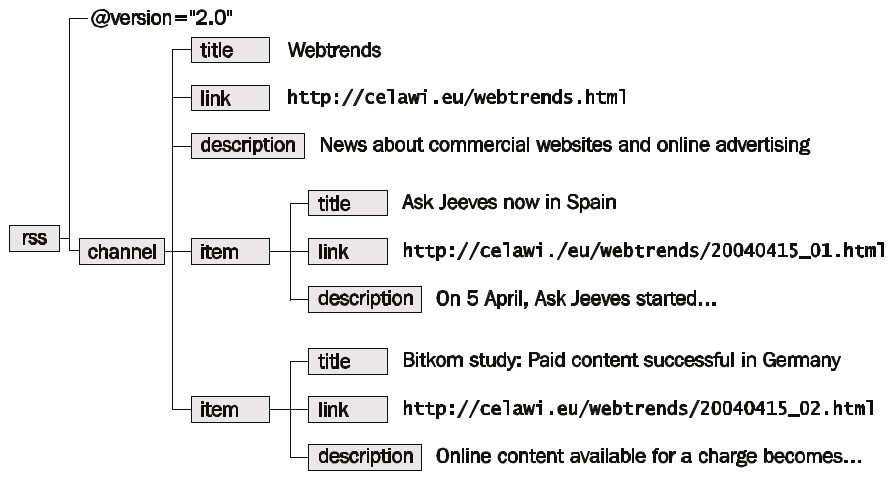
\includegraphics[scale=0.6]{structureRss}
	}
	\caption{Estructura de un documento RSS simple como un diagrama de árbol}
	\source{fuente: \cite{wittenbrink2005rss}}
	\label{fig:Estructura de un documento RSS simple como un diagrama de árbol}
\end{figure}


\subsection{Plataforma educativa LAEL}

En la figura \ref{fig:Suscriptor programa aprendizaje inglés básico}, se
muestra la acción de suscripción a una categoría (inglés básico) de un
usuario de sistema, con respecto al usuario tiene que iniciar sesión dentro 
del sistema. 

\begin{figure}[!ht]
	\centering
	\fbox{
		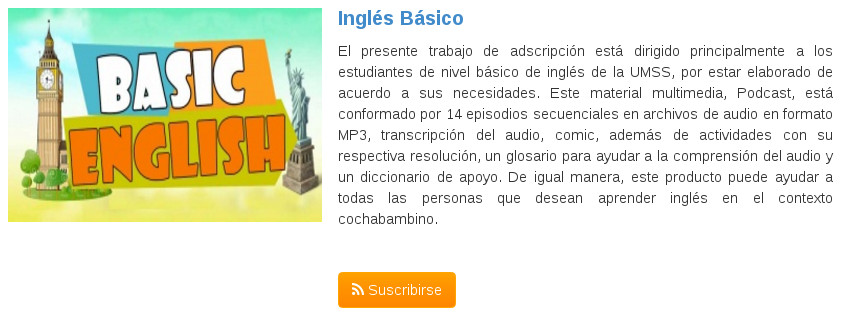
\includegraphics[scale=0.6]{basicEnglishSubscribe}
	}
	\caption{Suscriptor programa aprendizaje inglés básico}
	\source{fuente: (Elaboración propia)}
	\label{fig:Suscriptor programa aprendizaje inglés básico}
\end{figure}

En la figura \ref{fig:Presentación de un canal de noticia}, se muestra la
representación de un feed de la categoría inglés básico se utiliza un lector
desde la web. La estructura de un feed de noticia contempla título, fecha
para liberación y descripción.
 
\begin{figure}[!ht]
	\centering
	\fbox{
		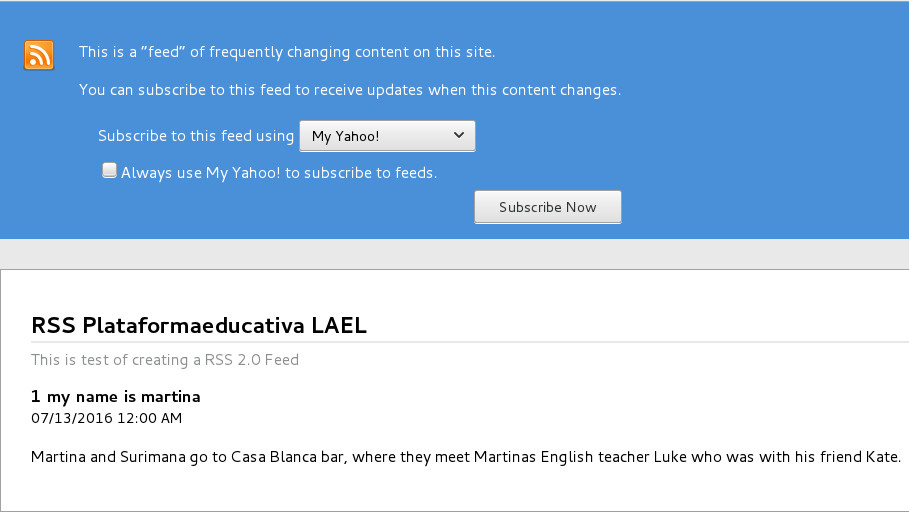
\includegraphics[scale=0.5]{basicEnglishRssFirefox}
	}
	\caption{Presentación de un canal de noticia}
	\source{fuente: (Elaboración propia)}
	\label{fig:Presentación de un canal de noticia}
\end{figure}

\section{El nuevo estándar atom}

Atom es otro tipo de feed compuesto por una serie de items
conocido como entry.

\subsection{Información básica de atom}

La estructura de un feed se describe a continuación.

\begin{itemize}

\item \textbf{title} contiene el título de la fuente de noticia.
\item \textbf{author} incluye información sobre el autor.
\item \textbf{updated} indica la última fecha de actualización.
\item \textbf{link} hace referencia a una versión diferente del contenido
y de la URI de atom.

\end{itemize}

La estructura de un entry se describe a continuación.

\begin{itemize}

\item \textbf{title} contiene el título de la fuente de noticia.
\item \textbf{summary} resumen del texto.
\item \textbf{updated} indica la última fecha de actualización.
\item \textbf{id} contiene una URI que identifica de forma única el feed.

\end{itemize}

En definitiva estos elementos son obligatorios de un elemento feed. Si esta
información no se encuentra presente, un documento atom es considerado no
válido. \cite{wittenbrink2005rss}

En la figura \ref{fig:Estructura de un documento Atom}, se presenta la
estructura de un documento atom representado de forma gráfica.

\begin{figure}[!ht]
\centering
	\fbox{
		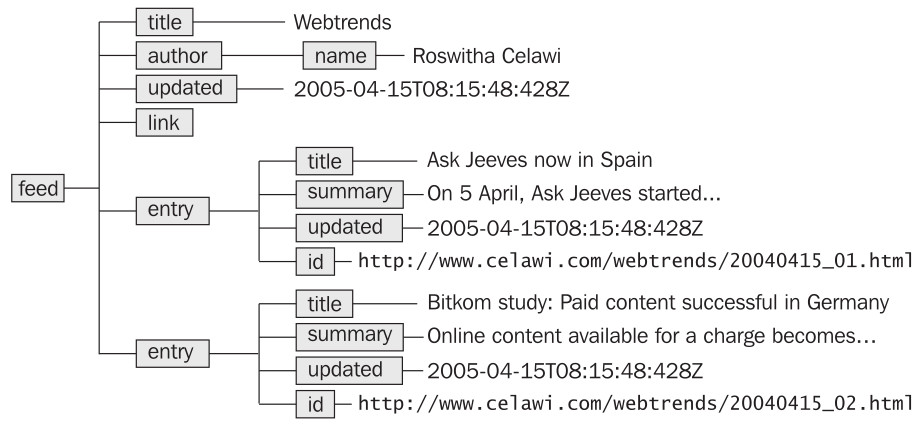
\includegraphics[scale=0.6]{structureAtom}
	}
	\captionof{figure}{Estructura de un documento Atom}
	\source{fuente: \cite{wittenbrink2005rss}}
	\label{fig:Estructura de un documento Atom}
\end{figure}
